\subsection{Space Vector Pulse Width Modulation}

Space Vector PWM has several advantages over Sine PWM

\begin{itemize}
	\item Higher voltage utilization: SVPWM can utilize up to 15\% more DC bus voltage compared to SPWM. This means for the same DC supply voltage, an inverter with SVPWM can provide a higher output voltage.

	\item Better harmonic performance: SVPWM results in lower total harmonic distortion (THD) compared to SPWM. This leads to a better quality of the output voltage and current waveforms, which is particularly important in applications like drives where harmonics can cause heating and torque pulsations.

	\item Reduced switching losses: SVPWM requires fewer switching operations for the inverter switches compared to SPWM. This results in lower switching losses, leading to higher efficiency and reduced heating of the inverter switches.

	\item Improved dynamic response: The space vector representation used in SVPWM allows for a more precise control of the output voltage vector, leading to an improved dynamic response. This is particularly beneficial in applications like motor drives where a fast dynamic response is required.

	\item Vector control capability: SVPWM allows for vector control of the output voltage, which is not possible with SPWM. This enables more complex control strategies, such as field-oriented control (FOC), which can provide better performance in applications like motor drives.

	\item Flexibility: SVPWM allows for flexible control of the output voltage magnitude and frequency, as well as the phase relationship between the output voltage and current. This flexibility makes it suitable for a wide range of applications.
\end{itemize}

\subsubsection{Generation of Space Vector PWM with C2000 microcontroller}

To generate space vector PWM wave for the switches C2000 series microcontroller offers a hardware level module called ePWM or enhanced PWM module. It enables to generate PWM waves with high flexibility.

To generate symmetrical waveform, the ePWM's internal timer is configured in up-down count mode.

\subsubsection{PWM Frequency Calculation}

\subsection*{Variable Definitions}

\renewcommand{\arraystretch}{1.5}
\begin{tabular}{|>{\bfseries}l|l|}
	\hline
	Symbol      & Description                                 \\ \hline
	$F_{PWM}$   & Frequency of PWM (Hz)                       \\ \hline
	$T_{PWM}$   & Time period of PWM (seconds)                \\ \hline
	$TBCLK$     & Time base clock (Hz)                        \\ \hline
	$T_{TBCLK}$ & Time period of time base clock (in seconds) \\ \hline
	$TBPRD$     & Timer period (in clock cycles)              \\ \hline
	$EPWMCLK$   & ePWM module clock (in Hz)                   \\ \hline
	$HSPCLKDIV$ & High speed clock divider                    \\ \hline
	$CLKDIV$    & Clock divider                               \\ \hline
\end{tabular}

\vspace{0.2in}

The period of the PWM signal can be calculated using the formula:
\[
	T_{\text{PWM}} = 2 \times TBPRD \times T_{\text{TBCLK}}
\]
where \( TBPRD \) is the time base period.

\subsection{PWM Frequency (\( F_{\text{PWM}} \))}
The frequency of the PWM signal is defined as the inverse of the PWM period:
\[
	F_{\text{PWM}} = \frac{1}{T_{\text{PWM}}}
\]

\subsection{Time Base Clock (\( T_{\text{TBCLK}} \))}
The time base clock is given by:
\[
	T_{\text{TBCLK}} = \frac{\text{EPWMCLK}}{\text{HSPCLKDIV} \times \text{CLKDIV}}
\]
\begin{itemize}
	\item \( \text{EPWMCLK} \) is the clock frequency dedicated to the PWM module.
	\item \( \text{HSPCLKDIV} \) and \( \text{CLKDIV} \) are the dividers for the high-speed PWM clock.
\end{itemize}

\subsection{Timer Period (\( TBPRD \))}

\[
	TBPRD = {T_{\text{PWM}} \over 2 \times T_{\text{TBCLK}}}
\]

According to the FSAM20SH60A datasheet, a 15 kHz switching frequency is recommended for optimal performance. The dividers \( \text{HSPCLKDIV} \) and \( \text{CLKDIV} \) are both set to 1. Given that the EPWMCLK is derived from the system clock (SYSCLK) which operates at 200 MHz, the time base clock can be calculated as follows:

Given the PWM period \( T_{\text{PWM}} \) and the TBCLK frequency \( T_{\text{TBCLK}} \), we need to solve for \( TBPRD \) (Time Base Period Register). The calculations are as follows:

\begin{enumerate}
	\item \textbf{Calculation of \( T_{\text{PWM}} \):}
	      \[
		      T_{\text{PWM}} = \frac{1}{15 \times 10^3} \text{ seconds}
	      \]
	      This represents the period of the PWM.

	\item \textbf{Calculation of \( T_{\text{TBCLK}} \):}
	      \[
		      TBCLK = \frac{200 \times 10^6}{1 \times 1} = 200 \times 10^6 \text{ Hz}
	      \]
	      This is the frequency of the TBCLK (Time Base Clock).

	\item \textbf{Solving for \( TBPRD \):}
	      With \( T_{\text{PWM}} \) and \( T_{\text{TBCLK}} \) known, we get $6667$.
\end{enumerate}


Figure \ref{fig:svpwm_block} below shows the ePWM block in Simulink, which is used generate PWM waveforms from microcontroller.

\begin{figure}[H]
	\centering
	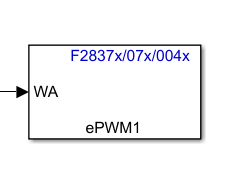
\includegraphics[width=1.8in]{sections/section6/images/SVPWM/ePWMBlock.png}
	\caption{ePWM block in Simulink}
	\label{fig:svpwm_block}
\end{figure}

Figure \ref{fig:ePWMTBPRD} below shows the ePWM module configuration.

\begin{figure}[H]
	\centering
	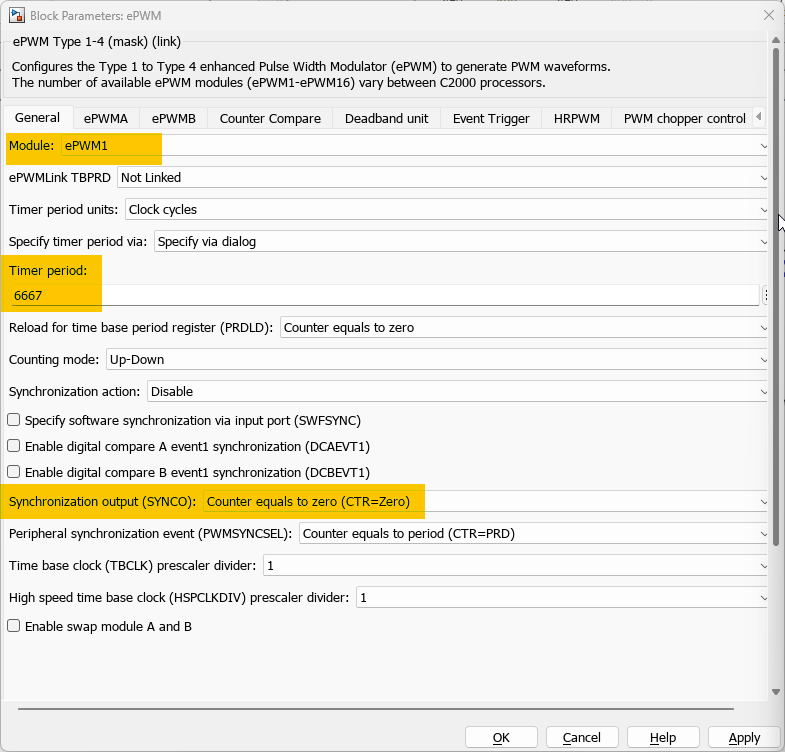
\includegraphics[width=4.3in]{sections/section6/images/SVPWM/ePWMTBPRD.png}
	\caption{ePWM configuration in Simulink}
	\label{fig:ePWMTBPRD}
\end{figure}

\subsubsection{Output of SVPWM with low pass filter}


The fundamental low frequency wave is buried within the 15 kHz carrier wave. Thus passed through a low pass filter to extract the fundamental frequency and hardware setup is shown in Figure \ref{fig:hardwareSetupLPF}.

\begin{figure}[H]
	\centering
	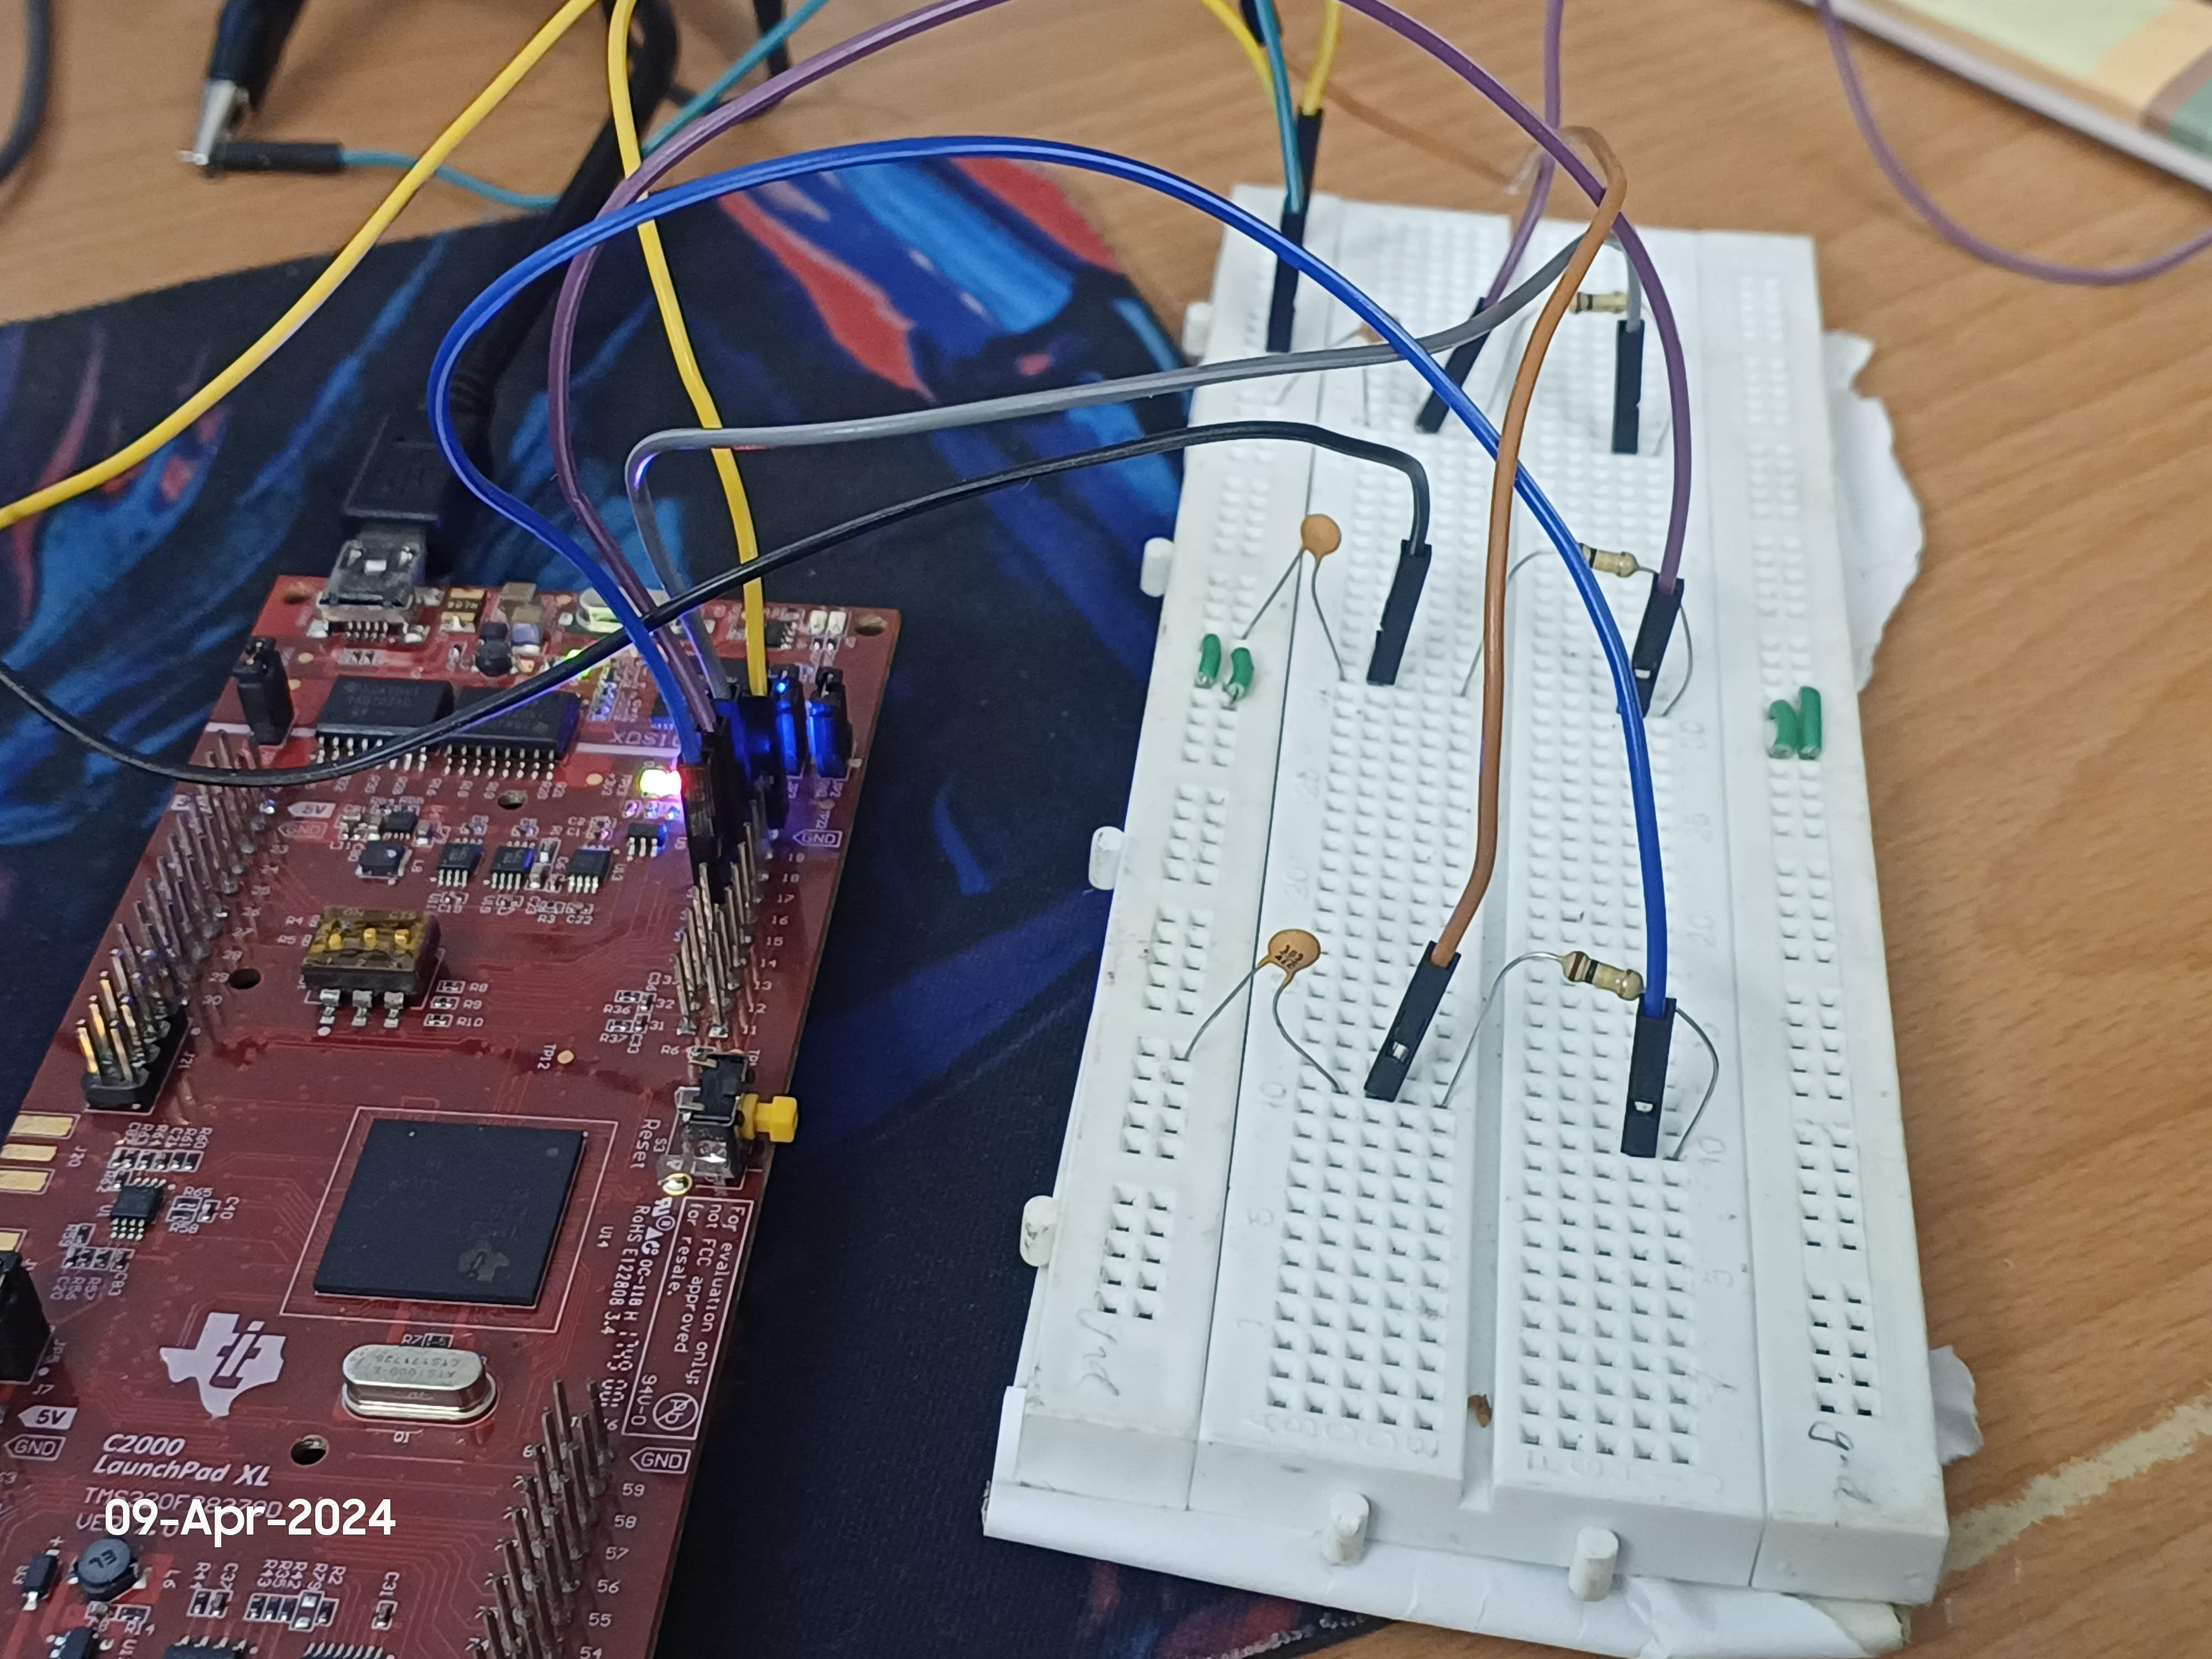
\includegraphics[width=4.3in]{sections/section6/images/SVPWM/LPFandC2000.jpg}
	\caption{Hardware setup with RC filter and Launchpad}
	\label{fig:hardwareSetupLPF}
\end{figure}

The output of the SVPWM with low pass filter is shown in Figure \ref{fig:OutputLPF}. The output is a SVPWM wave of 2 phases with a frequency 3hz.


\begin{figure}[H]
	\centering
	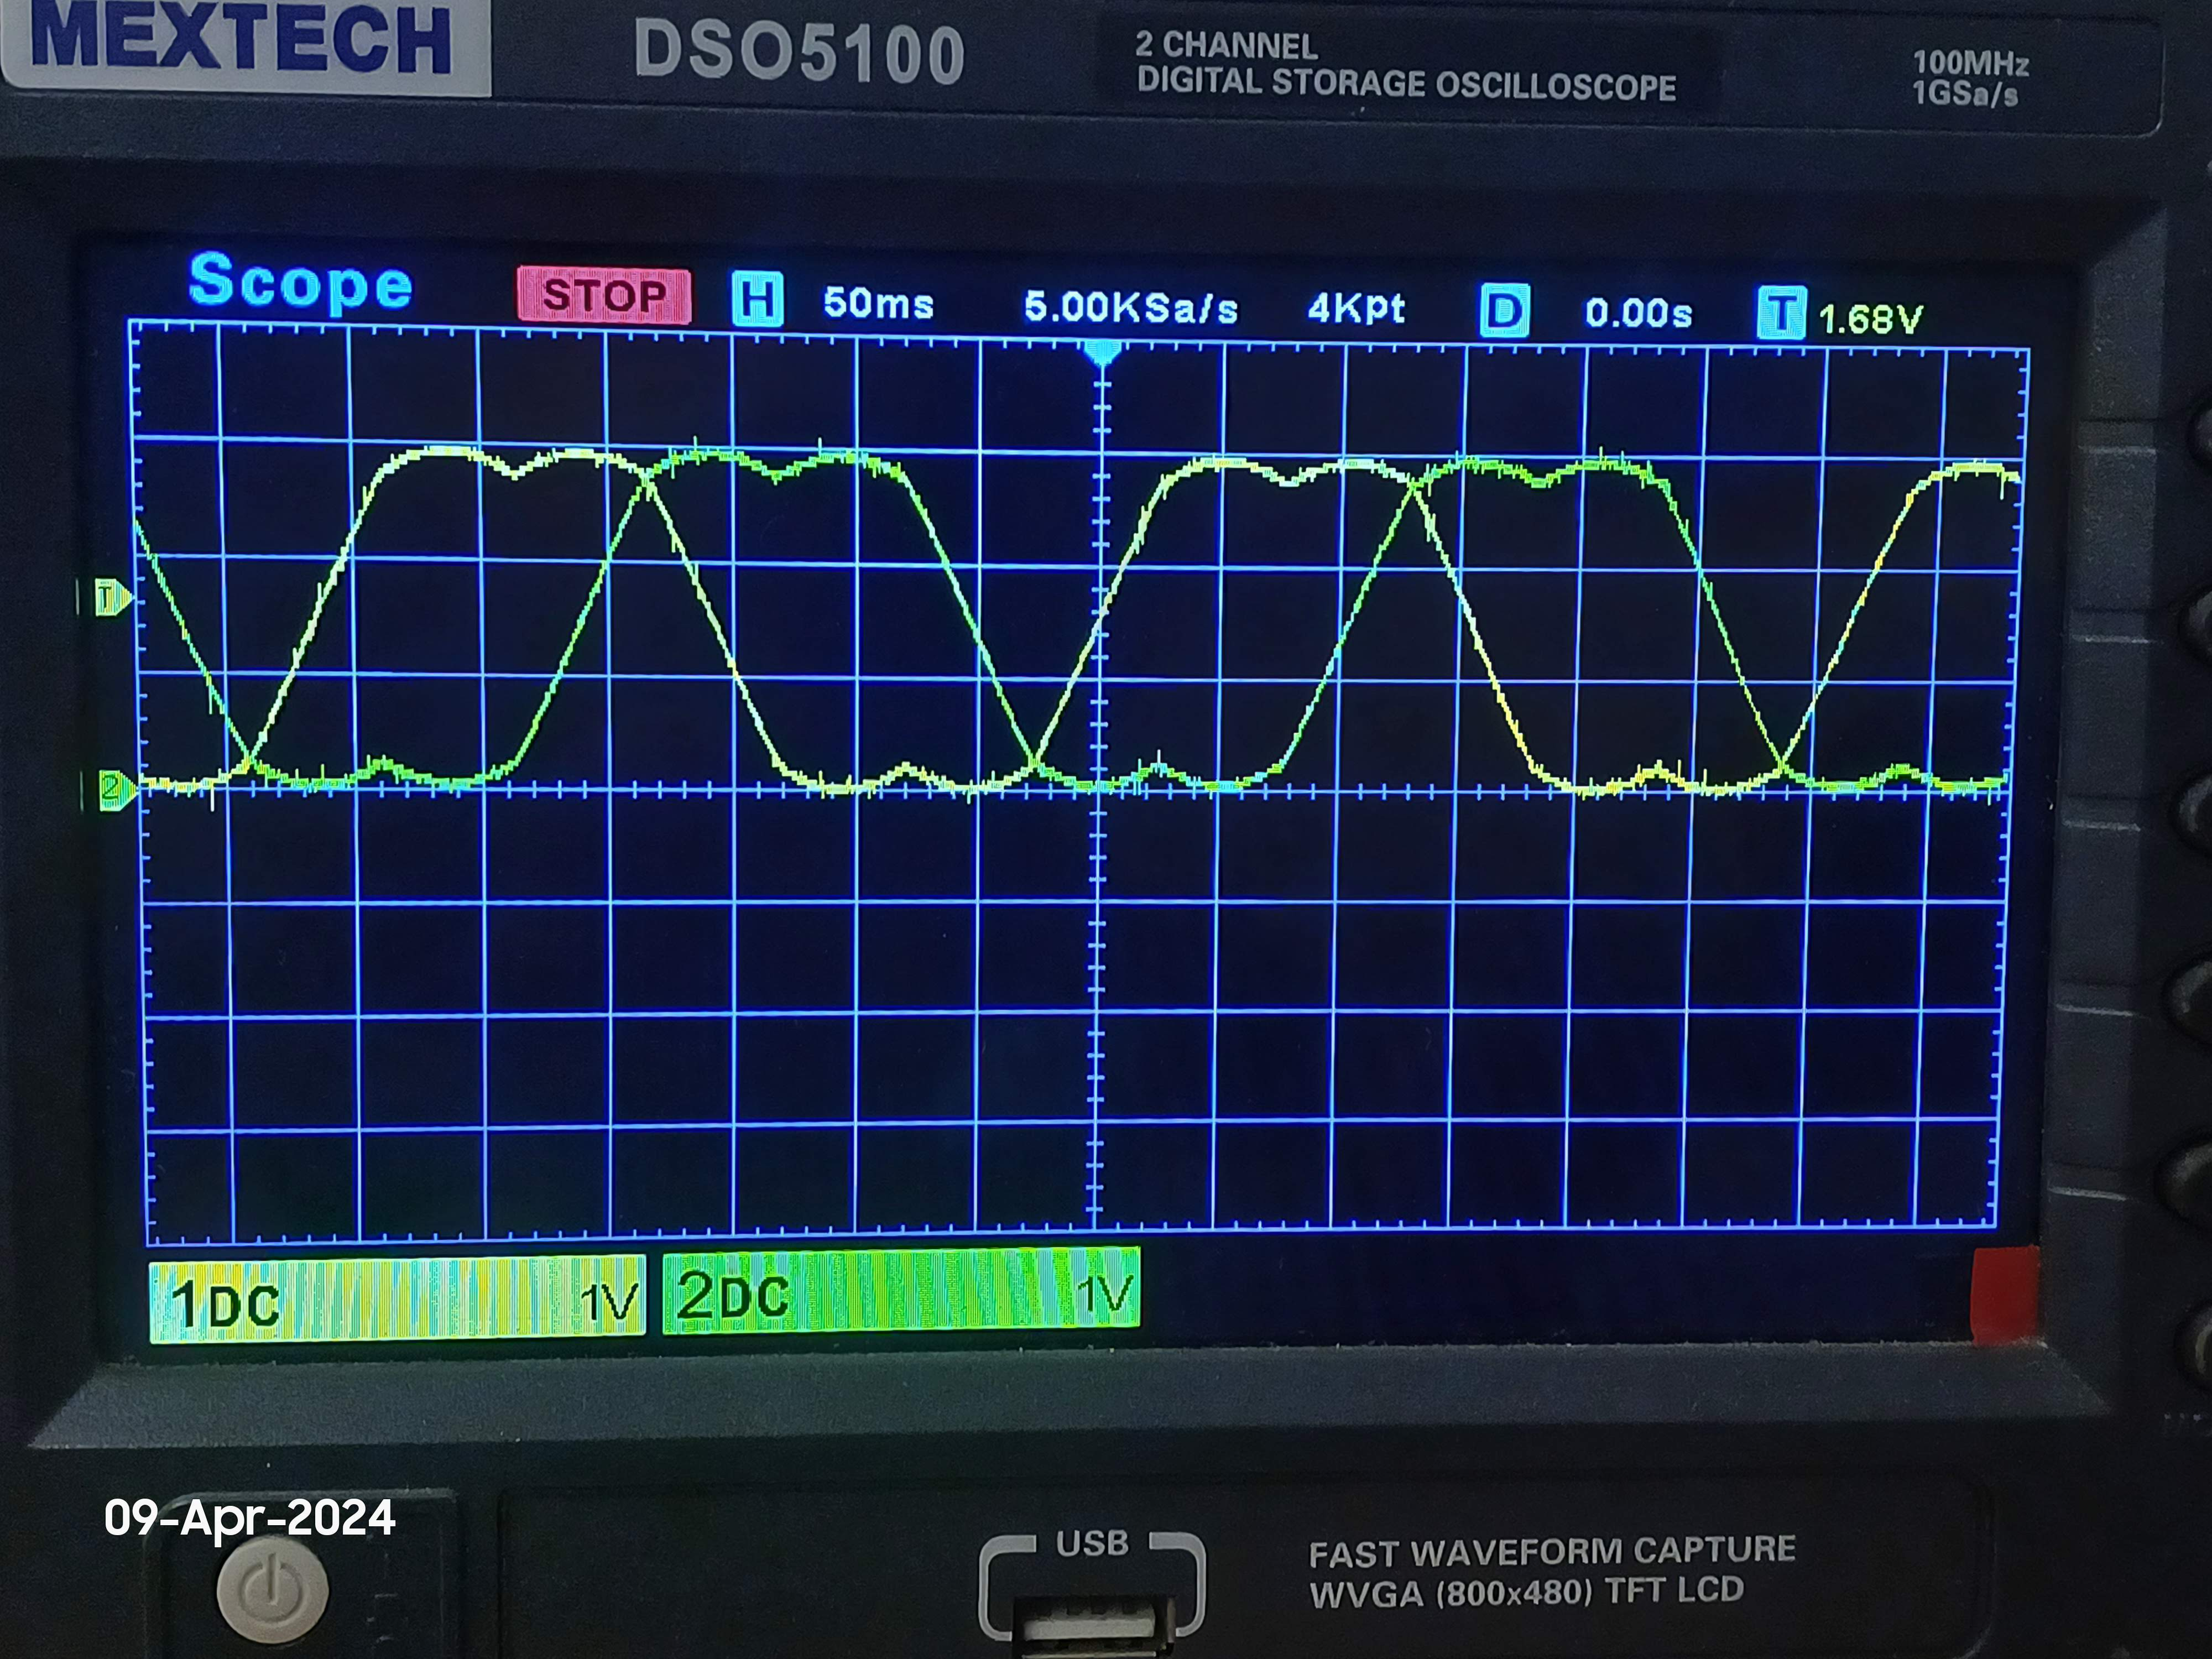
\includegraphics[width=4.3in]{sections/section6/images/SVPWM/SVPWM2phases.jpg}
	\caption{Output of SVPWM with low pass filter}
	\label{fig:OutputLPF}
\end{figure}


\subsubsection{Dead band}

Dead band is a time delay between the switching of the upper and lower switches in the inverter. This is necessary to prevent short circuiting of the DC bus. The dead band time is set in the ePWM module. The dead band time can be configured in the ePWM module, and it can be specified in terms of the number of clock cycles or in terms of time. The datasheet of FSAM20SH60A smart power module recommends a dead band time of atleast 3us.


\vspace{0.2in}

An example of 20us dead band time is shown in Figure \ref{fig:deadBand}. The two waveforms shown are output of ePWM 1A and 1B which will be given to the upper and lower switches of the inverter respectively.

\begin{figure}[H]
	\centering
	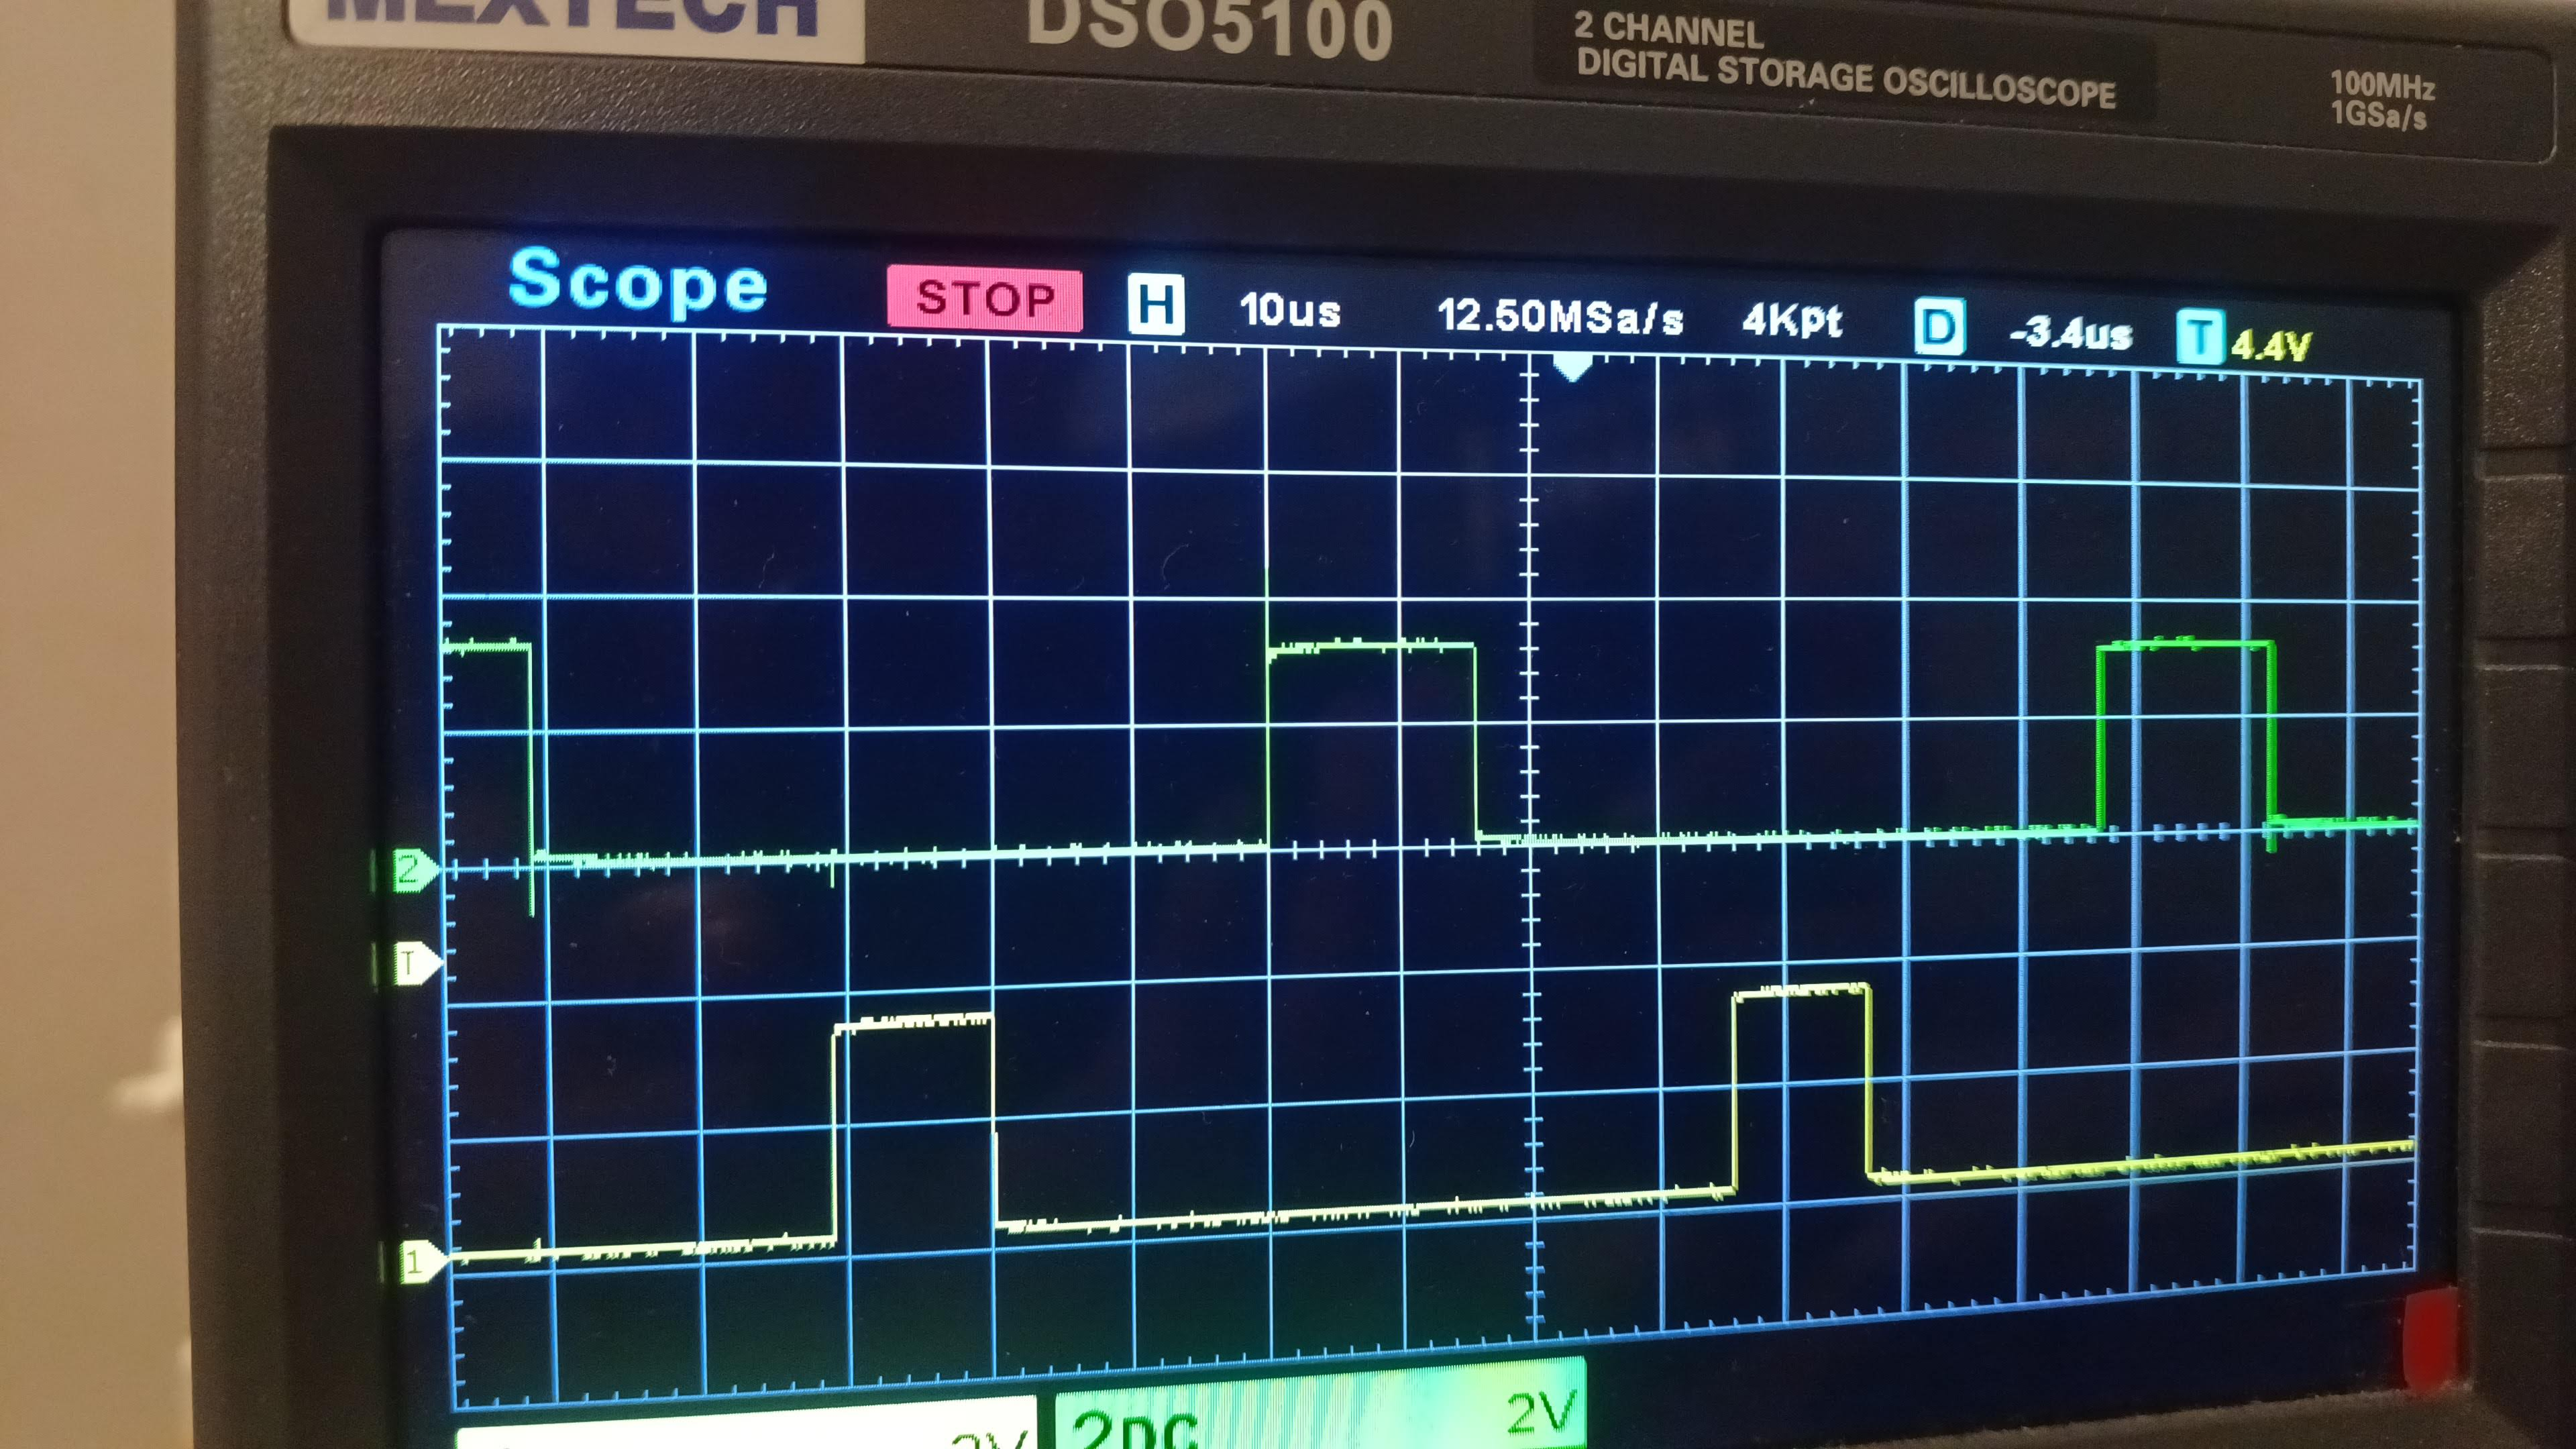
\includegraphics[width=4.3in]{sections/section6/images/SVPWM/DeadBand20Us.jpeg}
	\caption{Dead band time}
	\label{fig:deadBand}
\end{figure}


\newpage